\documentclass[a4paper,oneside]{article}
\usepackage[a4paper, margin=2cm, lmargin=2.5cm, rmargin=2.5cm, bmargin=1.2cm]{geometry}
\headsep=5pt
\usepackage{amsmath}
\usepackage{amsthm}
\usepackage{amsfonts}
\usepackage{xeCJK}       %讓中英文字體分開設置

\setCJKmainfont{Noto Sans CJK TC}
\XeTeXlinebreaklocale "zh"             %這兩行一定要加,中文才能自動換行
\XeTeXlinebreakskip = 0pt plus 1pt

\usepackage{enumitem}
\usepackage{algpseudocode}
\usepackage{tikz}
% Tikz settings optimized for causal graphs.
% Just copy-paste this part
\usetikzlibrary{shapes,decorations,arrows,calc,arrows.meta,fit,positioning}
\tikzset{
    -Latex,auto,node distance =1 cm and 1 cm,semithick,
    state/.style ={ellipse, draw, minimum width = 0.7 cm},
    point/.style = {circle, draw, inner sep=0.04cm,fill,node contents={}},
    bidirected/.style={Latex-Latex,dashed},
    el/.style = {inner sep=2pt, align=left, sloped}
}
\usepackage{listings}
\usepackage[T1]{fontenc}
\usepackage{fancyhdr}
\usepackage{url}
\usepackage{color}
\usepackage{graphicx}
\usepackage{tgcursor}
\usepackage[compact]{titlesec}
\titlespacing{\section}{0pt}{*0}{*0}
\titlespacing{\subsection}{0pt}{*0}{*0}
\titleformat{\section}[hang]
  {\normalfont\bfseries}
  {}
  {0em}
  {\Large \thesection\hspace{0.6em}}
\titleformat{\subsection}[hang]
  {\normalfont\bfseries}
  {}
  {0em}
  {\large \thesubsection\hspace{0.6em}}

\pagestyle{fancy}
\fancyfoot{}
\fancyhead[L]{Deep Learning and Practice}
\fancyhead[R]{Page \thepage}
\definecolor{deeper}{gray}{.8}

\renewcommand*{\ttdefault}{pcr}
\lstset{
		basicstyle=\footnotesize\ttfamily,
		tabsize=2,
		breaklines=true,
}
\setlist{leftmargin=\parindent}

\setlength{\parindent}{1em}
\graphicspath{ {./images/} }
\titlespacing{\section}{0pc}{1pc}{0.5pc}
\titlespacing{\subsection}{0pc}{1pc}{0.5pc}
\titlespacing{\subsubsection}{0pc}{1pc}{0.5pc}
\linespread{1.2}

\usepackage{dirtree}
\usepackage{hyperref}
\usepackage{subfig}

\begin{document}
\title{[Lab1] Back-propagation}
\author{0616014 楊政道}
\maketitle
\thispagestyle{fancy}
\section{Introduction}
\subsection{Lab Objective}
\paragraph{}
In this assignment, I will implement a simple neural network with both forward pass and back-propagation. The structure of the simple network will consist of fully-connected layers and sigmoid functions. The loss function will use mean squared error and the optimizer will use the stochastic gradient decent method.
\paragraph{}
Furthermore, I will try different activation functions, loss functions and optimizers to make the network converged better and faster with some experimental verification.
\subsection{Project Structure}
\dirtree{%
.1 Lab1\_0616014.zip.
.2 dataset/.
.3 displayer.py.
.3 generator.py.
.3 processor.py.
.2 model/.
.3 function/.
.4 activation.py.
.4 loss.py.
.3 network.py.
.3 optimizer.py.
.3 structure.py.
}
\subsubsection{dataset/displayer.py}
\paragraph{}
There are some functions to display data including
\begin{itemize}
    \item line plot(error plot or accuracy plot)
    \item decision region plot
    \item comparison plot between ground truth and prediction
\end{itemize}
\begin{figure}[!ht]
\begin{center} 
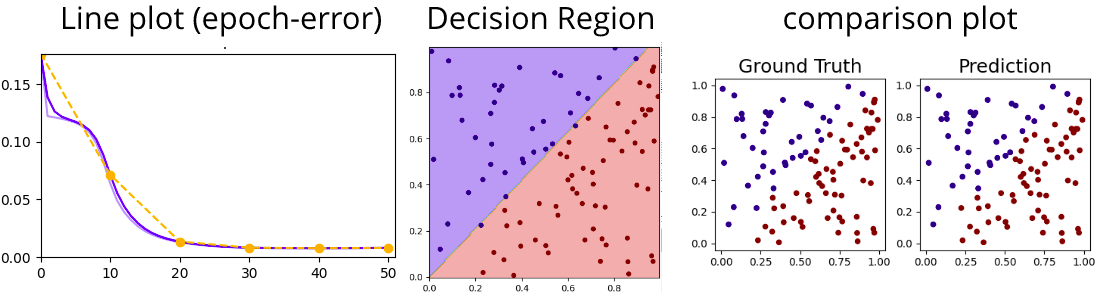
\includegraphics[width=15cm]{displayer-view.png} 
\caption{All kinds of displayers}
\end{center} 
\end{figure} 
\subsubsection{dataset/generator.py}
\paragraph{}
There are some classes to generate data including Linear, XOR and NSpirals(N is a variable).
\begin{figure}[!ht]
\begin{center} 
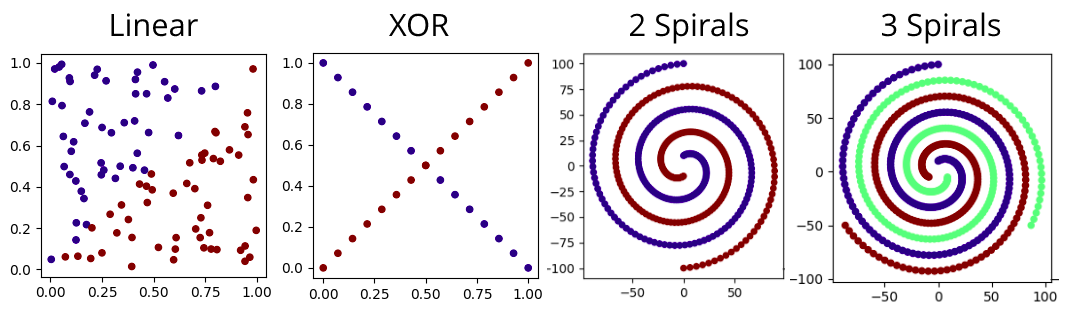
\includegraphics[width=15cm]{generator-view.png} 
\caption{All kinds of generators}
\end{center} 
\end{figure} 
\subsubsection{dataset/processor.py}
\paragraph{}
There are some data handlers about one-hot encoder and decoder, data shuffling handler.
\subsubsection{model/function/activation.py}
\paragraph{}
There are some classes about activation functions layers including Sigmoid, ReLu(Leaky ReLu) and SoftMax.
\subsubsection{model/function/loss.py}
\paragraph{}
There are some classes about loss functions including mean squared error and binary cross entropy.
\subsubsection{model/network.py}
\paragraph{}
There is a class about neural networks to make the network construction easier.
\subsubsection{model/optimizer.py}
\paragraph{}
There are some classes about optimizers including SGD and Adam.
\subsubsection{model/structure.py}
\paragraph{}
There is a class about network structures including FullyConnectedLayer.
\section{Experimental Setup}
\subsection{Fully Connected Layers}
\begin{lstlisting}[language=Python]
class FullyConnected:

    def __init__(self, m, n):
        self.W = np.random.uniform(-1, 1, (m + 1, n)).astype('float128')

    def forward(self, X):
        self.X = np.concatenate((
            X, np.array([ 1 for x in X ]).reshape(-1, 1)
        ), axis=1)
        return np.dot(self.X, self.W)

    def backward(self, E, optimizer):
        return optimizer.update(self, E)
\end{lstlisting}
\paragraph{}
A \texttt{m} to \texttt{n} fully-connected layer is a \texttt{m + 1} by \texttt{n} matrix (weight and bias). Its forward pass is just a dot operation with input matrix. When updating the fully-connected layer, we can call the update function of its optiomizer.
\subsection{Sigmoid Function}
\begin{lstlisting}[language=Python]
class Sigmoid:

    def evaluate(self, X):
        return 1 / (1 + np.exp(-X))

    def gradient(self, X):
        return self.evaluate(X) * (1 - self.evaluate(X))

    def forward(self, X):
        self.X = X
        return self.evaluate(X)
        
    def backward(self, E, optimizer):
        return self.gradient(self.X) * E
\end{lstlisting}
\paragraph{}
An activation function contains two basic functions, evaluate and gradient. They correspond to defination and differential of sigmoid function.
$$\text{Sigmoid}(x) = \frac{1}{1 + e^{-x}}$$
$$\frac{\partial \text{Sigmoid}(x)}{\partial x}=\text{Sigmoid}(x)(1 - \text{Sigmoid}(x))$$
\paragraph{}
Then, its forward pass is to call evaluate function and its backward pass is to call gradient function and times the error passed from previous layer.
\subsection{Mean Squared Error}
\begin{lstlisting}[language=Python]
class MeanSquaredError:

    def evaluate(self, Y_hat, Y):
        return (Y - Y_hat) ** 2 / 2.0

    def gradient(self, Y_hat, Y):
        return - (Y - Y_hat)
\end{lstlisting}
\paragraph{}
A loss function contains two basic functions which are similar to activation functions. They correspond to defination and differential of mean squared error.
$$\text{MSE}(y, \hat{y}) = \frac{1}{2}(y - \hat{y})^2$$
$$\frac{\partial \text{MSE}(y, \hat{y})}{\partial \hat{y}} = -(y - \hat{y})$$
\subsection{Optimizer}
\begin{lstlisting}[language=Python]
class SGD:

    def __init__(self, lr=0.01):
        self.lr = lr

    def update(self, layer, E):
        gradient = np.dot(layer.X.T, E)
        E = np.dot(E, layer.W.T)[:, :-1]
        layer.W -= self.lr * gradient
        return E
\end{lstlisting}
\paragraph{}
An optimizer need to update weight of layers and pass the error to the next layers.
\subsection{Neural Network}
\begin{lstlisting}[language=Python]
class Network:

    def __init__(self, structure, optimizer, loss):
        self.structure = structure
        self.optimizer = optimizer
        for layer in self.structure:
            self.optimizer.initial(layer)
        self.loss = loss
\end{lstlisting}
\paragraph{}
Input structure, optimizer and loss to define a network. A structure list will be like this below.
\begin{lstlisting}[language=Python]
structure = [
    FullyConnected(2, 5),
    Sigmoid(),
    FullyConnected(5, 5),
    Sigmoid(),
    FullyConnected(5, 2),
    Sigmoid()
]
\end{lstlisting}
\subsubsection{Forward Pass}
\begin{lstlisting}[language=Python]
class Network:

    def forward(self, Y):
        for layer in self.structure:
            Y = layer.forward(Y)
        return Y
\end{lstlisting}
Forward pass of the network is just to go through forward functions of all layers and return the result value.
\subsubsection{Back-propagation}
\begin{lstlisting}[language=Python]
class Network:

    def backward(self, E):
        for layer in self.structure[::-1]:
            E = layer.backward(E, self.optimizer)
\end{lstlisting}
\paragraph{}
Backward pass of the network is to go through backward functions of all layers in the reversed order and update weight with optimizer.
\subsubsection{Train}
\begin{lstlisting}[language=Python]
class Network:

    def train(self, X, Y, epochs = 10):
        for epoch in range(epochs):
            for x, y in zip(X, Y):
                x = x.reshape(1, -1)
                y = y.reshape(1, -1)
                y_hat = self.forward(x)
                self.backward(self.loss.gradient(y_hat, y))
\end{lstlisting}
\paragraph{}
Training function of the network is to do a forward and a backward pass for all data pairs with severals epochs.
\section{Experimental Result}
\subsection{Linear}
\subsubsection{Network Settings}
\begin{lstlisting}[language=Python]
# dataset
dataset = Linear()
dataset_num = 100

# network
network_structure = [
    FullyConnected(2, 3),
    Sigmoid(),
    FullyConnected(3, 3),
    Sigmoid(),
    FullyConnected(3, 2),
    Sigmoid(),
]

# train
epochs = 50
optimizer = SGD(0.5)
loss = MeanSquaredError()
\end{lstlisting}

\subsubsection{Experimental Result}
\begin{figure}[!ht]
    \centering
    \subfloat[comparsion plot]{{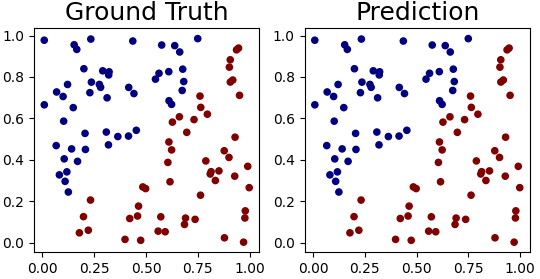
\includegraphics[width=10cm]{linear_v1-gt_pd.png} }}
    \qquad
    \subfloat[decision region]{{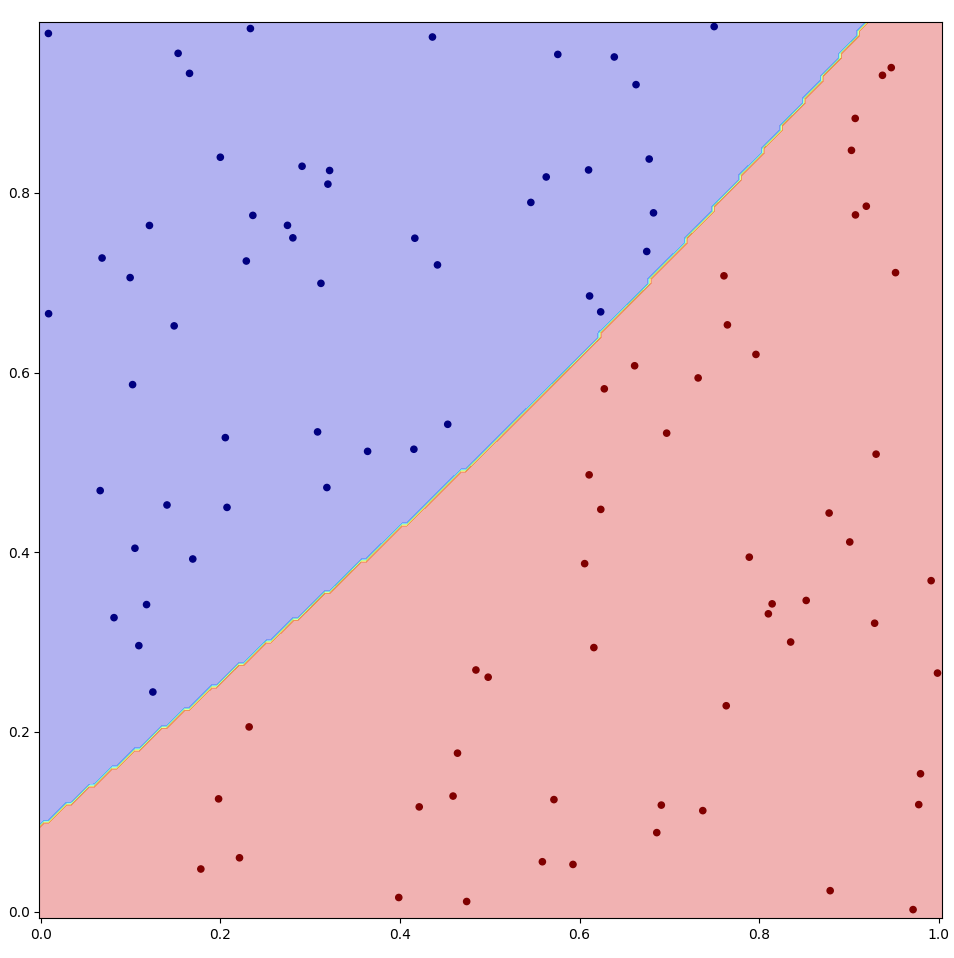
\includegraphics[width=5cm]{linear_v1-decision_region.png} }}
    \qquad
    \subfloat[accuracy plot]{{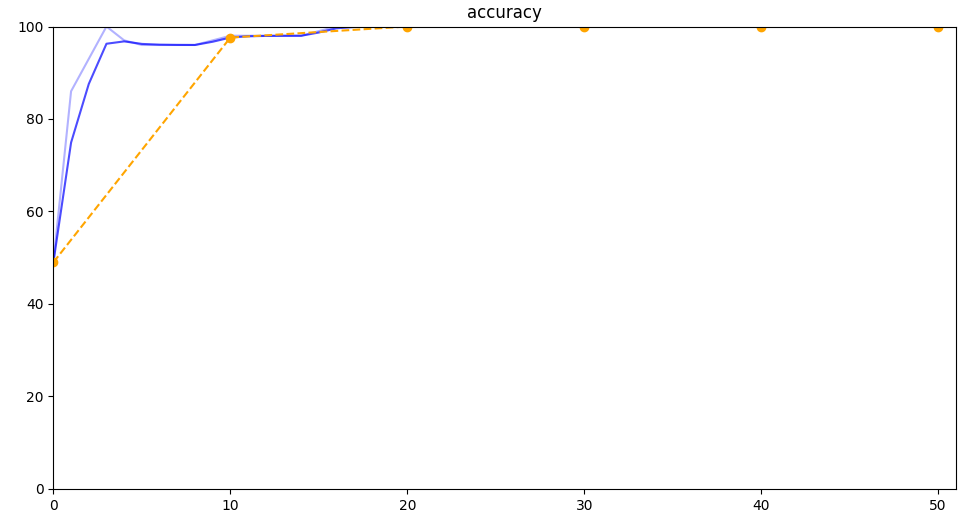
\includegraphics[width=7cm]{linear_v1-acc.png} }}
    \qquad
    \subfloat[error plot]{{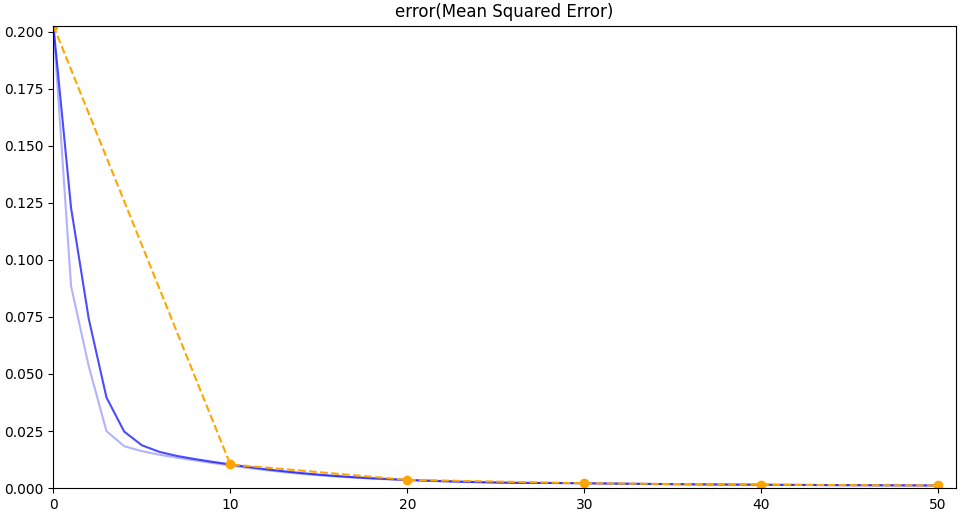
\includegraphics[width=7cm]{linear_v1-err.png}}}
    \caption{linear}
\end{figure}
\newpage
\subsection{XOR}
\subsubsection{Network Settings}
\begin{lstlisting}[language=Python]
# dataset
dataset = XOR()
dataset_num = 50

# network
network_structure = [
    FullyConnected(2, 8),
    Sigmoid(),
    FullyConnected(8, 8),
    Sigmoid(),
    FullyConnected(8, 2),
    Sigmoid(),
]

# train
epochs = 200
optimizer = SGD(1)
loss = MeanSquaredError()
\end{lstlisting}

\subsubsection{Experimental Result}
\begin{figure}[!ht]
    \centering
    \subfloat[comparsion plot]{{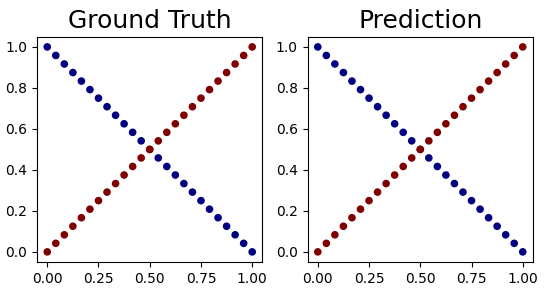
\includegraphics[width=10cm]{xor_v1-gt_pd.png} }}
    \qquad
    \subfloat[decision region]{{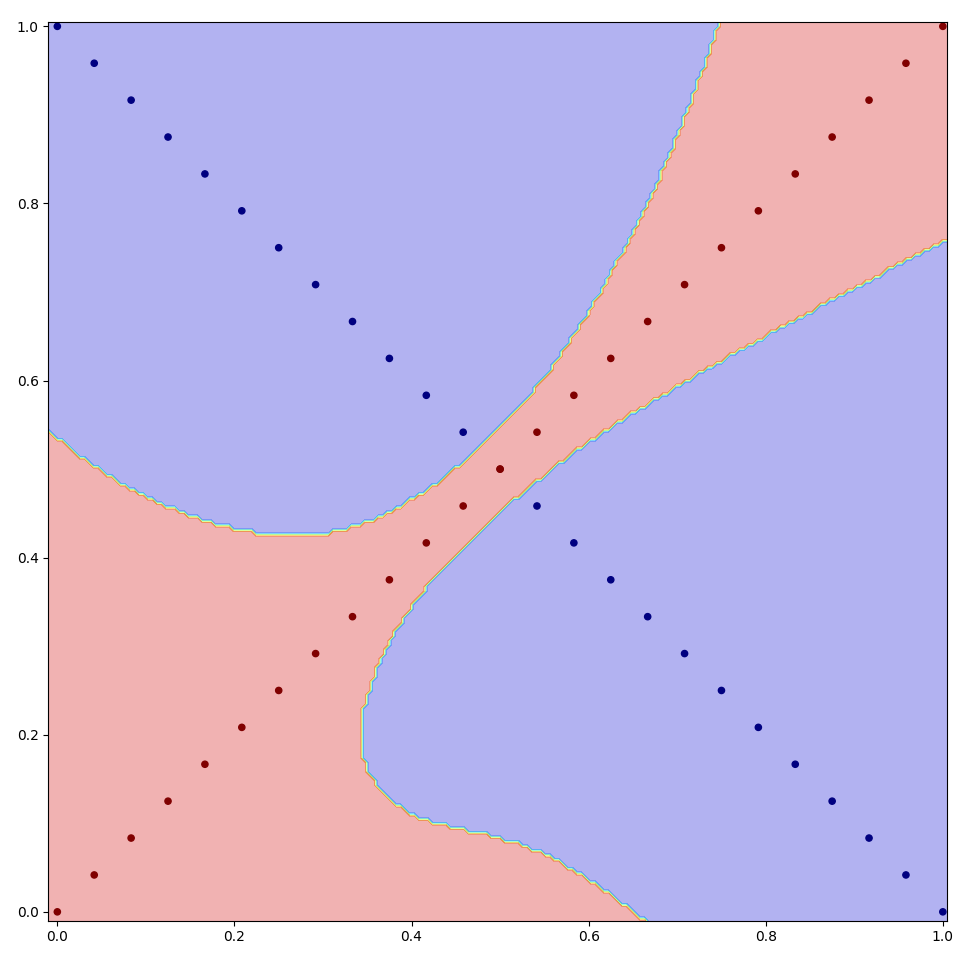
\includegraphics[width=5cm]{xor_v1-decision_region.png} }}
    \qquad
    \subfloat[accuracy plot]{{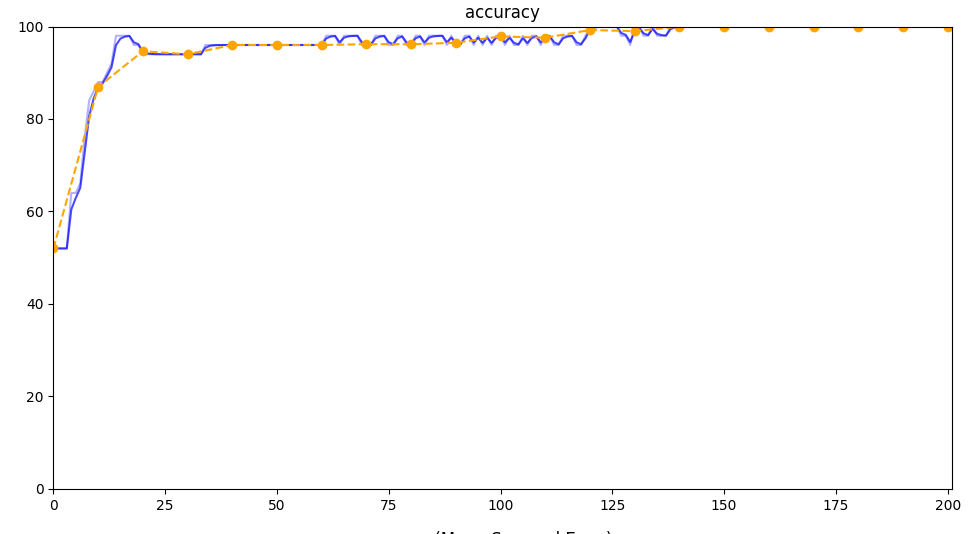
\includegraphics[width=7cm]{xor_v1-acc.png} }}
    \qquad
    \subfloat[error plot]{{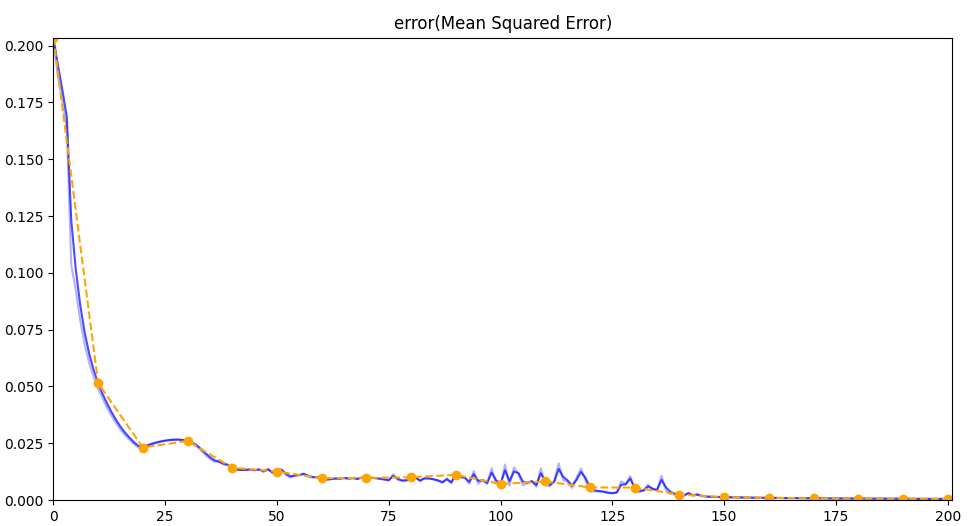
\includegraphics[width=7cm]{xor_v1-err.png}}}
    \caption{xor}
\end{figure}

\newpage
\section{Discussion}
\subsection{Activation Function - Sigmoid and Others}
\subsubsection{Sigmoid}
\paragraph{}
Sigmoid function has two fatal problems
\begin{enumerate}
    \item The computation of the exponential function is costly and slow.
    \item The gradient shrinks when the input value is far from the zero. 
\end{enumerate}
\begin{figure}[!ht]
\begin{center} 
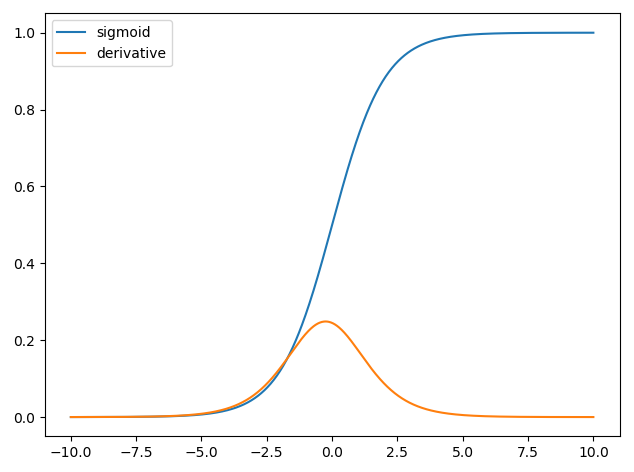
\includegraphics[width=5cm]{sigmoid.png} 
\caption{sigmoid function}
\end{center} 
\end{figure}
\paragraph{}
Therefore, we need to find a kind of activation function which doesn't have high-computation operation and gradient shrinking. 
\subsubsection{ReLu}
\paragraph{}
ReLu activation function improves the disadvantage of the sigmoid function memtioned above. It doesn't have any exponential operations and the gradient doesn't shrink for the large input value.
\begin{figure}[!ht]
\begin{center} 
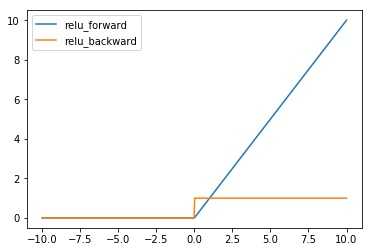
\includegraphics[width=5cm]{relu.jpg} 
\caption{relu function}
\end{center} 
\end{figure}
\begin{lstlisting}[language=Python]
class ReLu:

    def __init__(self, r):
        self.r = r

    def evaluate(self, X):
        return X * (X > 0) + self.r * (X < 0) * X

    def gradient(self, X):
        return 1 * (X > 0) + self.r * (X < 0)

    def forward(self, X):
        self.X = X
        return self.evaluate(X)

    def backward(self, E, optimizer):
        return self.gradient(self.X) * E
\end{lstlisting}
\paragraph{}
However, when we replace the activation function of the last layer, the range of the output value will not be bounded in (0, 1). Therefore, we need another activation function to bound the range of the output value.

\subsubsection{SoftMax}
\paragraph{}
We can use softmax function to make the range of the output value into (0, 1).
$$\text{Softmax}(x_{i}) = \frac{\exp(x_i)}{\sum_j \exp(x_j)}$$
\begin{lstlisting}[language=Python]
class SoftMax:

    def evaluate(self, X):
        X = X - np.max(X, axis=1).reshape(-1, 1)
        e_X = np.exp(X)
        return e_X / np.sum(e_X, axis=1).reshape(-1, 1)

    def gradient(self, X):
        return self.evaluate(X).T * (np.identity(X.shape[1]) - self.evaluate(X))

    def forward(self, X):
        self.X = X
        return self.evaluate(X)

    def backward(self, E, optimizer):
        return np.dot(E, self.gradient(self.X))
\end{lstlisting}
\paragraph{}
The gradient of the softmax activation function is more complex than other activation functions.
$$\frac{\partial \text{softmax}(x_i)}{\partial x_i} = \text{softmax}(x_i)(\mathbb{I}(i = j) - \text{softmax}(x_j))$$
\subsection{Loss Function}
\subsubsection{Mean Squared Error}
\paragraph{}
Mean squared error has a fatal error the gradient at the position close to zero is too smal to train. Therefore, when the late of the training stage, the network is hard to converge.
\subsubsection{Binary Cross Entropy}
\begin{lstlisting}[language=Python]
class BinaryCrossEntropy:

    def evaluate(self, Y_hat, Y):
        return - (Y * np.log(1e-9 + Y_hat) + (1 - Y) * np.log(1e-9 + 1 - Y_hat))

    def gradient(self, Y_hat, Y):
        return - (Y / (1e-9 + Y_hat) - (1 - Y) / (1e-9 + 1 - Y_hat))
\end{lstlisting}
\paragraph{}
A loss function contains two basic functions(evaluate and gradient). They correspond to defination and differential of binary cross entropy.
$$\text{BCE}(y, \hat{y}) = y \times log(\hat {y}) + (1 - y) \times log(1 - \hat{y})$$
$$\frac{\partial \text{BCE}(y, \hat{y})}{\partial \hat{y}} = \frac{y}{\hat{y}} - \frac{1 - y}{1 - \hat{y}}$$

\begin{figure}[!ht]
    \begin{center} 
    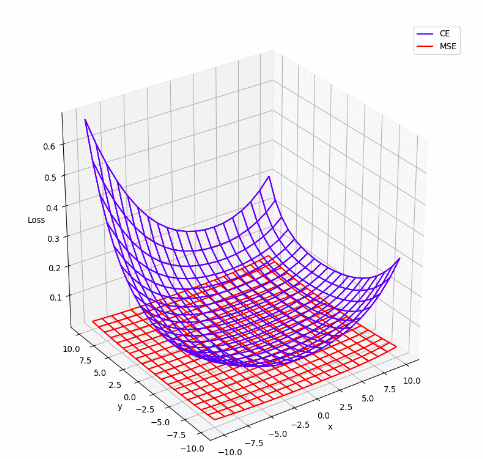
\includegraphics[width=7cm]{mse-ce.png} 
    \caption{mean squared error vs cross entropy}
    \end{center} 
\end{figure}
\newpage

\subsection{Optimizer}
\subsubsection{Stochastic Gradient Decent}
$$W \leftarrow  W - \eta \frac{\partial L}{\partial W}$$
\paragraph{}
Stochastic gradient decent has some fatal problems.
\begin{itemize}
    \item cannot do anything when stucking in local minimum.
    \item use the same learning rate to update all the elements of the weight.
\end{itemize}
\subsubsection{Adam}
\paragraph{}
Adam optimizer use $m$ and $v$ two variables to update weight. 
$$W \leftarrow W - \eta \frac{\hat{m}_t}{\sqrt{\hat{v}_t} + \epsilon}$$
\paragraph{About $m$}
\paragraph{}
Gradient desent is like putting a ball on a surface and the ball will fall into low. The ball will have the momentum so that it can slide out from the local minimum. Variable $m$ is like the momentum of the ball. For each iteration, it refer to past momentum like the inertia of the ball.
$$m_t = \beta_1m_{t-1} + (1 - \beta_1)\frac{\partial L_t}{\partial W_t}$$
\paragraph{About $v$}
\paragraph{}
The variable $v$ can make the sensitive parameters change less and the smoothing parameters change more, so that the whole parameters can be close to the optimized value at the same time without causing same parts to be prematurely trained but interfered by other parameters.
$$v_t = \beta_2v_{t-1} + (1 - \beta_2)(\frac{\partial L_t}{\partial W_t})^2$$
\paragraph{About decay}
\paragraph{}
When the late of the training stage, the learning rate will be more less than the begining of the training stage's. Therefore, we can use the following formula to make the change smaller and smaller over time.
$$\hat{m}_t = \frac{m_t}{1 - \beta_1^t}$$
$$\hat{v}_t = \frac{v_t}{1 - \beta_2^t}$$

\section{Extra Experiments}
\subsection{Linear with Advanced Model}
\subsubsection{Network Settings}
\begin{lstlisting}[language=Python]
# dataset
dataset = Linear()
dataset_num = 200

# network
network_structure = [
    FullyConnected(2, 5),
    ReLu(0.1),
    FullyConnected(5, 5),
    ReLu(0.1),
    FullyConnected(5, 2),
    SoftMax()
]

# train
epochs = 30
optimizer = Adam(0.1, 0.99)
loss = BinaryCrossEntropy()
\end{lstlisting}

\subsubsection{Experimental Result}
\begin{figure}[!ht]
    \centering
    \subfloat[comparsion plot]{{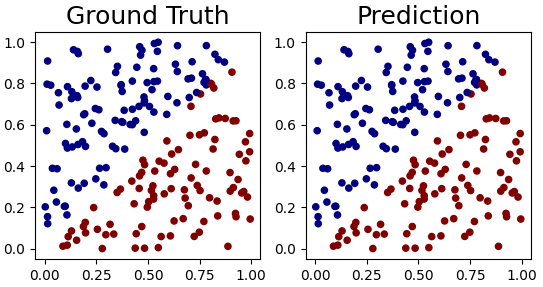
\includegraphics[width=10cm]{linear_v2-gt_pd.png} }}
    \qquad
    \subfloat[decision region]{{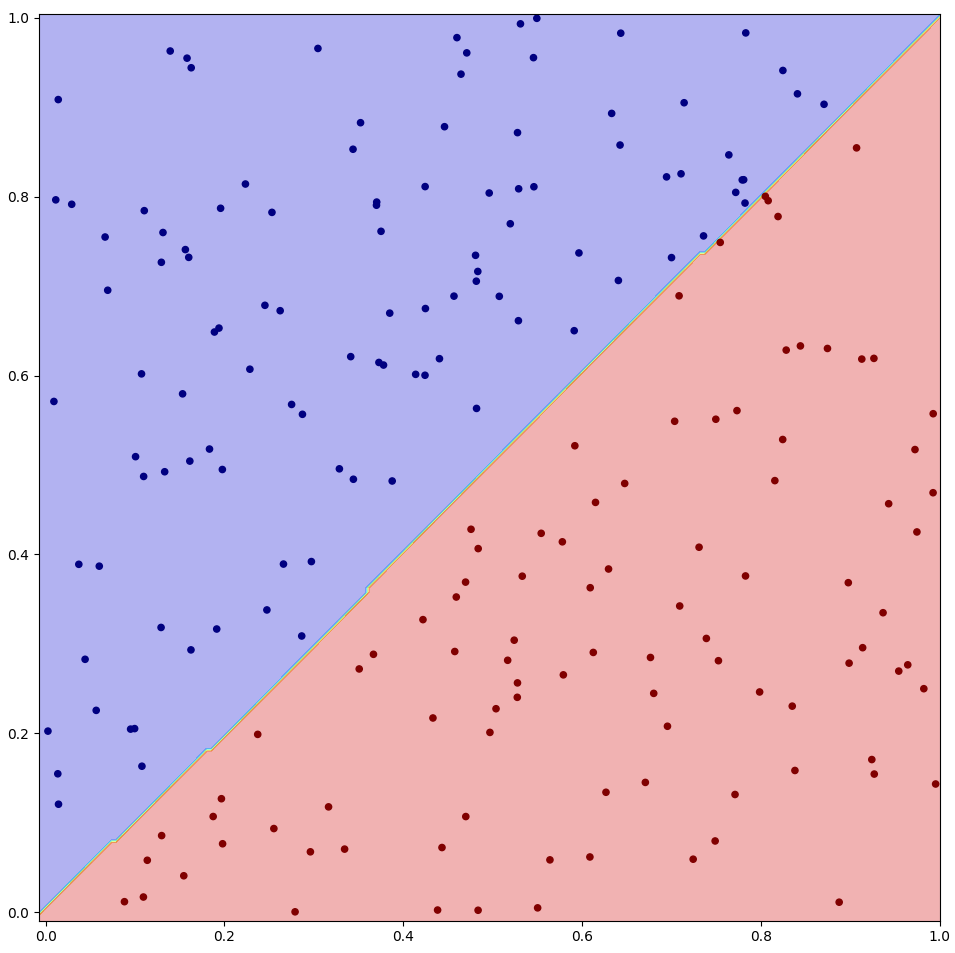
\includegraphics[width=5cm]{linear_v2-decision_region.png} }}
    \qquad
    \subfloat[accuracy plot]{{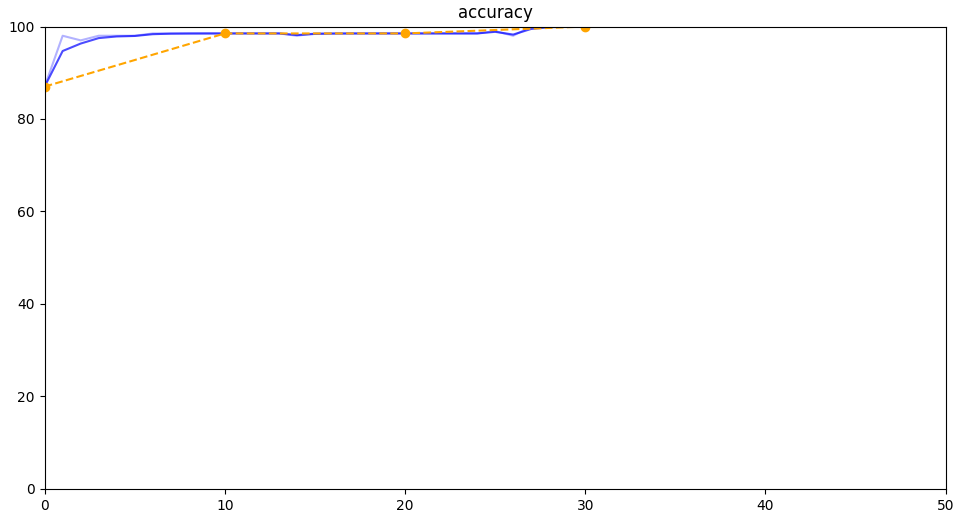
\includegraphics[width=7cm]{linear_v2-acc.png} }}
    \qquad
    \subfloat[error plot]{{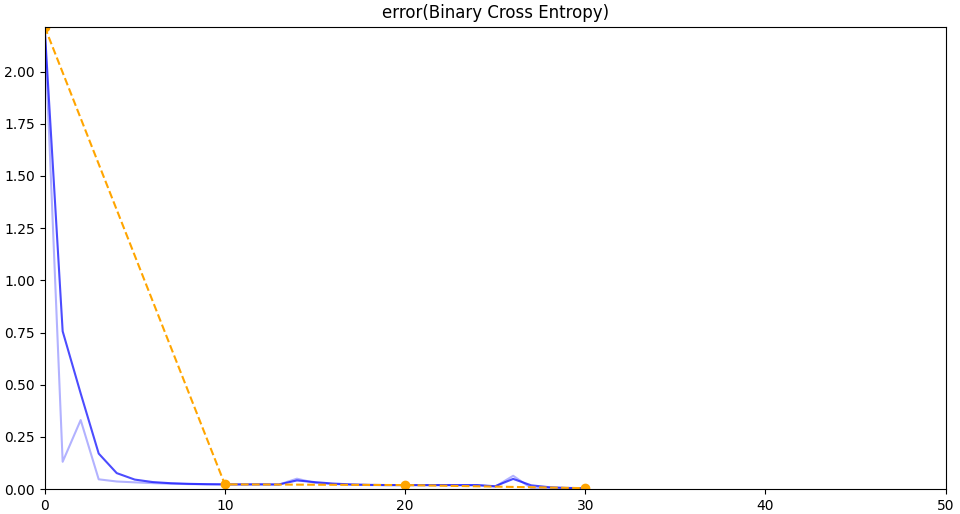
\includegraphics[width=7cm]{linear_v2-err.png}}}
    \caption{linear with advanced model}
\end{figure}

\newpage
\subsection{XOR with Advanced Model}
\subsubsection{Network Settings}
\begin{lstlisting}[language=Python]
# dataset
dataset = XOR()
dataset_num = 50

# network
network_structure = [
    FullyConnected(2, 5),
    ReLu(0.1),
    FullyConnected(5, 5),
    ReLu(0.1),
    FullyConnected(5, 2),
    SoftMax()
]

# train
epochs = 100
optimizer = Adam(0.1, 0.99)
loss = BinaryCrossEntropy()
\end{lstlisting}

\subsubsection{Experimental Result}
\begin{figure}[!ht]
    \centering
    \subfloat[comparsion plot]{{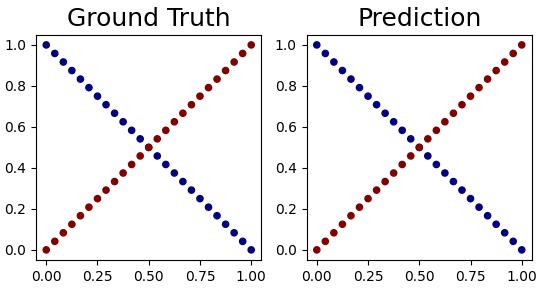
\includegraphics[width=10cm]{xor_v2-gt_pd.png} }}
    \qquad
    \subfloat[decision region]{{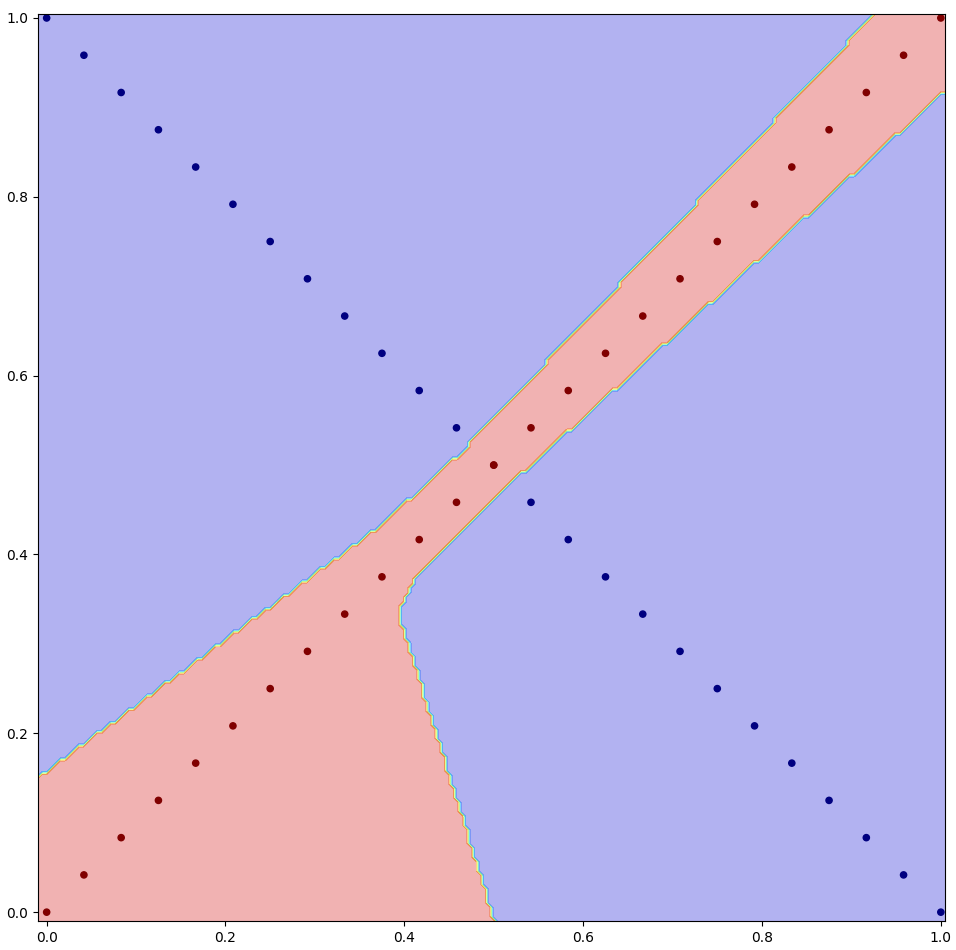
\includegraphics[width=5cm]{xor_v2-decision_region.png} }}
    \qquad
    \subfloat[accuracy plot]{{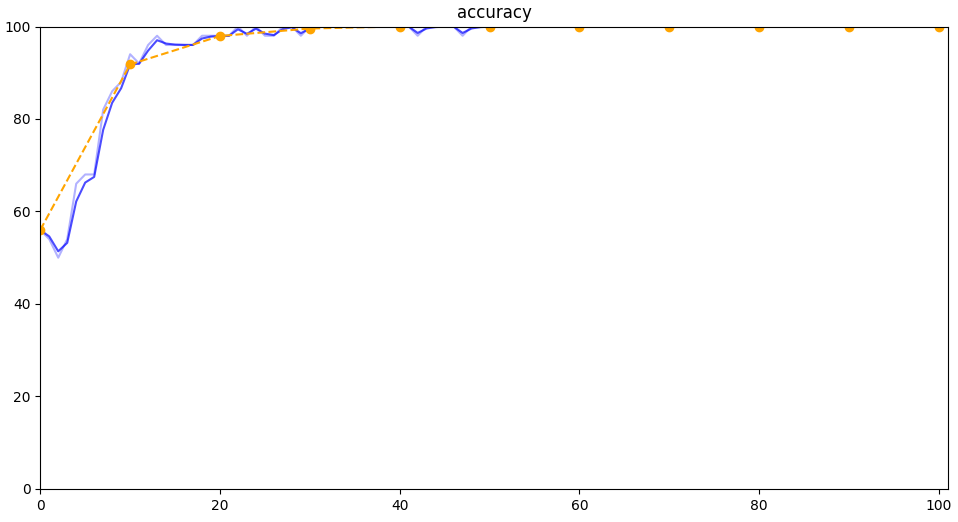
\includegraphics[width=7cm]{xor_v2-acc.png} }}
    \qquad
    \subfloat[error plot]{{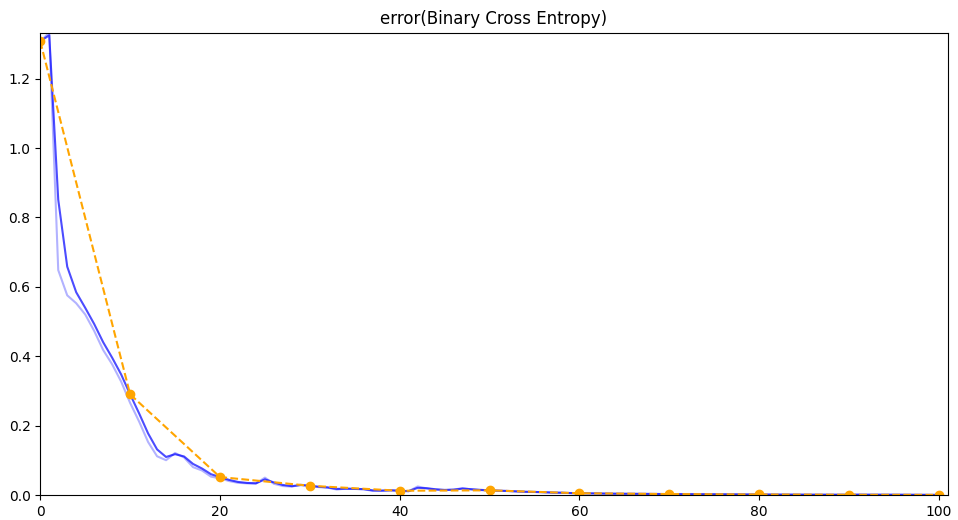
\includegraphics[width=7cm]{xor_v2-err.png}}}
    \caption{xor with advanced model}
\end{figure}

\newpage
\subsection{2 Circles with Advanced Model}
\subsubsection{Network Settings}
\begin{lstlisting}[language=Python]
# dataset
dataset = TwoCircles()
dataset_num = 500

# network
network_structure = [
    FullyConnected(2, 15),
    ReLu(0.1),
    FullyConnected(15, 15),
    ReLu(0.1),
    FullyConnected(15, 2),
    SoftMax()
]

# train
epochs = 30
optimizer = Adam(0.01, 0.99)
loss = BinaryCrossEntropy()
\end{lstlisting}

\subsubsection{Network Settings}
\begin{figure}[!ht]
    \centering
    \subfloat[comparsion plot]{{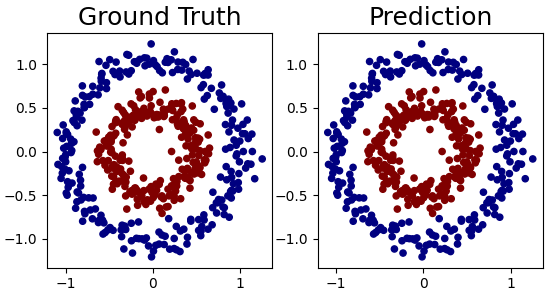
\includegraphics[width=10cm]{2circles-gt_pd.png} }}
    \qquad
    \subfloat[decision region]{{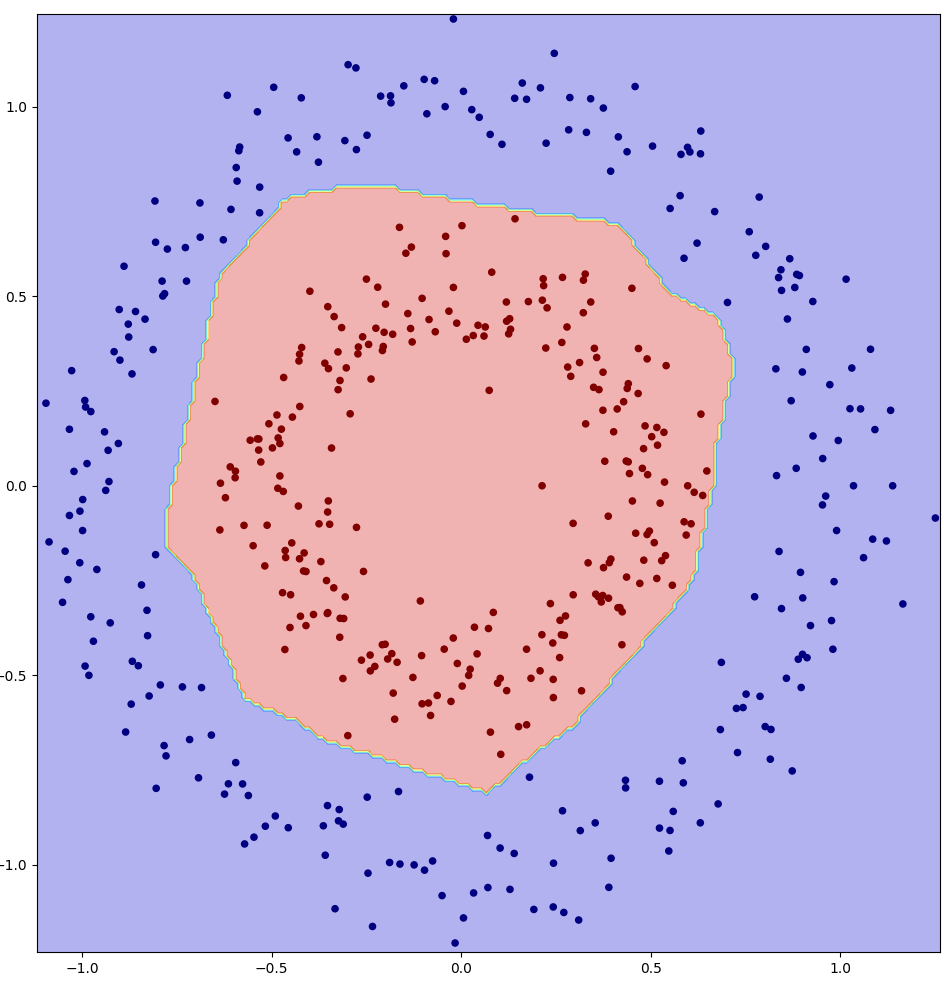
\includegraphics[width=5cm]{2circles-decision_region.png} }}
    \qquad
    \subfloat[accuracy plot]{{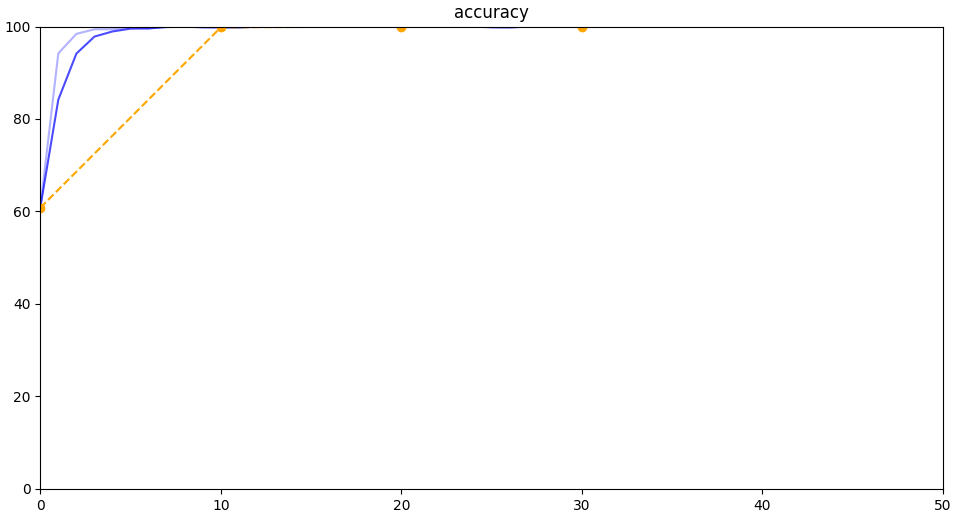
\includegraphics[width=7cm]{2circles-acc.png} }}
    \qquad
    \subfloat[error plot]{{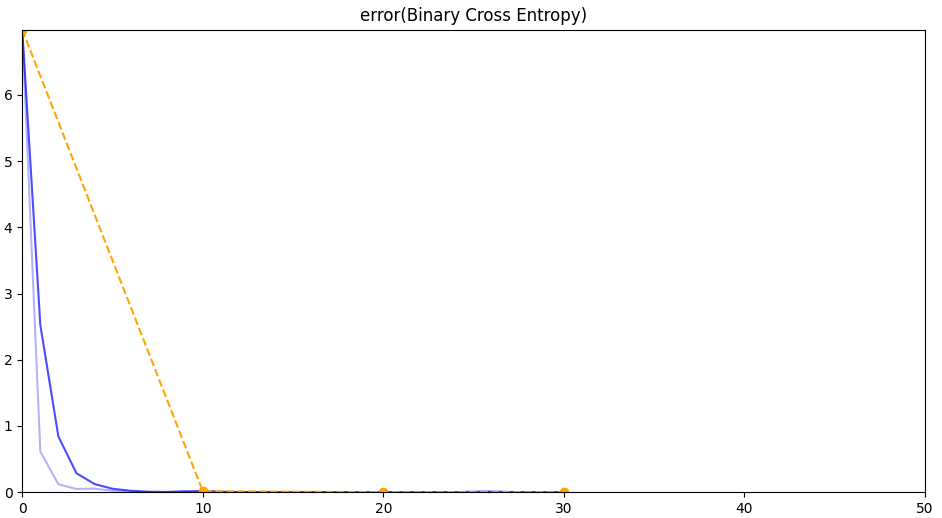
\includegraphics[width=7cm]{2circles-err.png}}}
    \caption{2 circles}
\end{figure}

\newpage
\subsection{2 Spirals with Advanced Model}
\subsubsection{Network Settings}
\begin{lstlisting}[language=Python]
# dataset
dataset = NSpirals(2)
dataset_num = 400

# network
network_structure = [
    FullyConnected(2, 10, -1, 1),
    ReLu(0.1),
    FullyConnected(10, 10, -1, 1),
    ReLu(0.1),
    FullyConnected(10, 2, -1, 1),
    SoftMax()
]

# train
epochs = 200
optimizer = Adam(0.01, 0.99)
loss = BinaryCrossEntropy()
\end{lstlisting}

\subsubsection{Experimental Result}
\begin{figure}[!ht]
    \centering
    \subfloat[comparsion plot]{{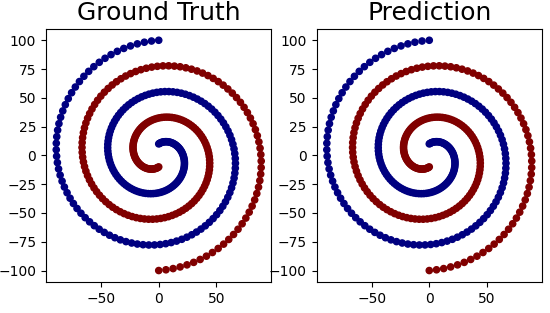
\includegraphics[width=10cm]{2spirals-gt_pd.png} }}
    \qquad
    \subfloat[decision region]{{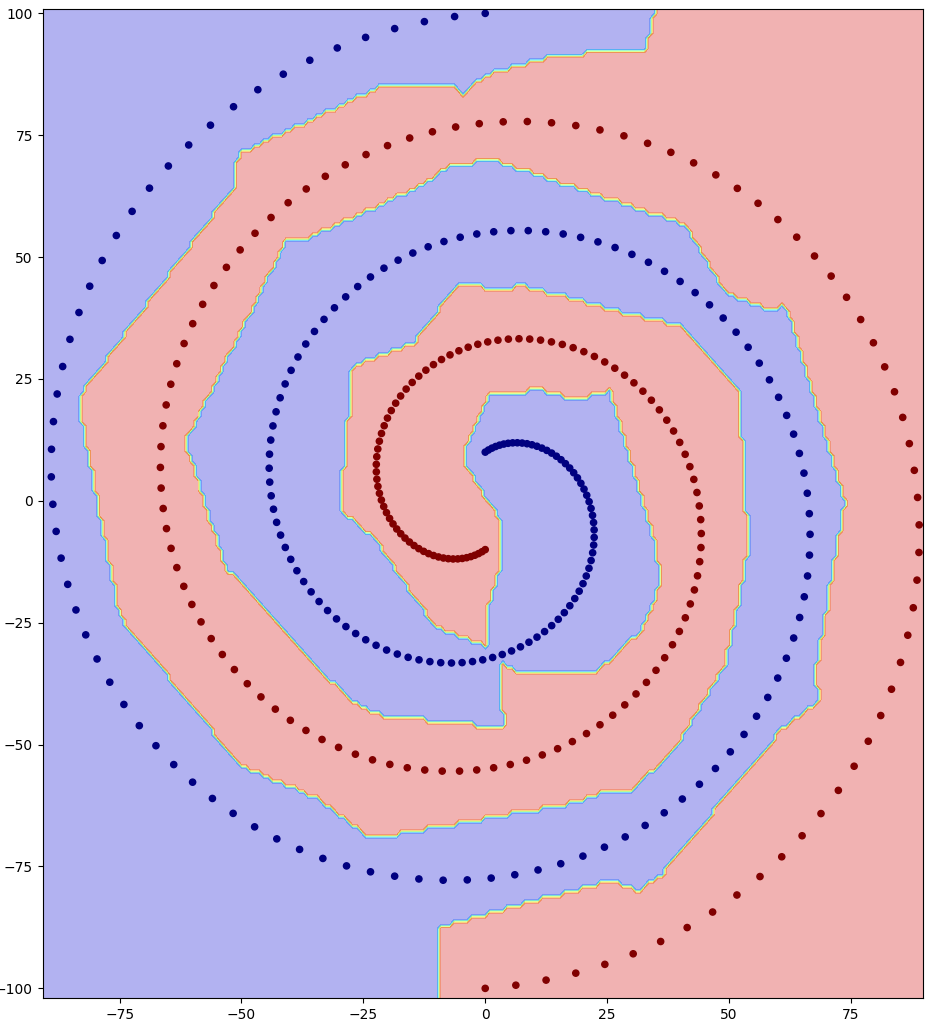
\includegraphics[width=5cm]{2spirals-decision_region.png} }}
    \qquad
    \subfloat[accuracy plot]{{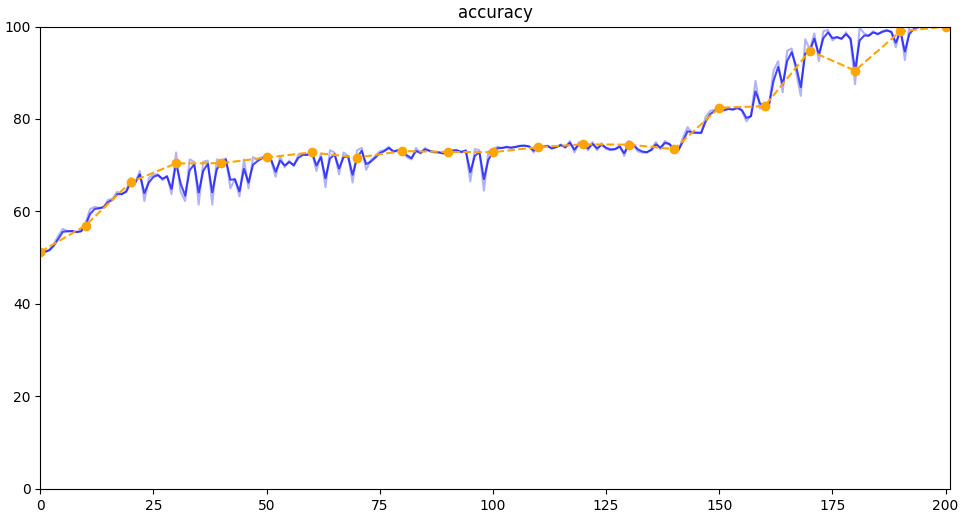
\includegraphics[width=7cm]{2spirals-acc.png} }}
    \qquad
    \subfloat[error plot]{{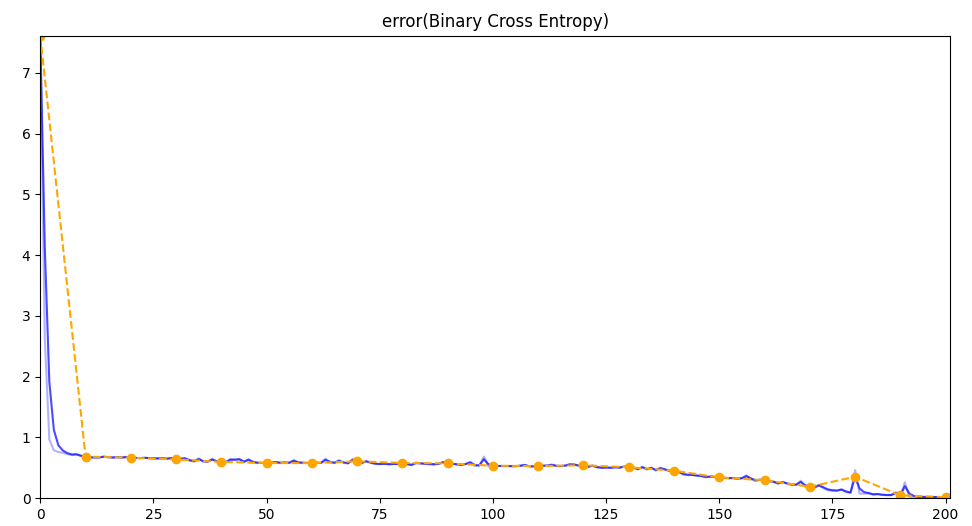
\includegraphics[width=7cm]{2spirals-err.png}}}
    \caption{2 spirals}
\end{figure}

\newpage
\subsection{3 Spirals with Advanced Model}
\subsubsection{Network Settings}
\begin{lstlisting}[language=Python]
# dataset
dataset = NSpirals(3)
dataset_num = 600

# network
network_structure = [
    FullyConnected(2, 15, -1, 1),
    ReLu(0.1),
    FullyConnected(15, 15, -1, 1),
    ReLu(0.1),
    FullyConnected(15, 3, -1, 1),
    SoftMax()
]

# train
epochs = 200
optimizer = Adam(0.01, 0.99)
loss = BinaryCrossEntropy()
\end{lstlisting}

\subsubsection{Experimental Result}
\begin{figure}[!ht]
    \centering
    \subfloat[comparsion plot]{{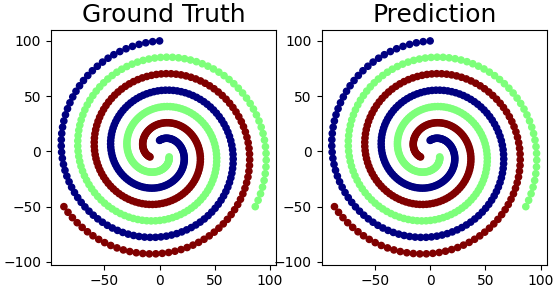
\includegraphics[width=10cm]{3spirals-gt_pd.png} }}
    \qquad
    \subfloat[decision region]{{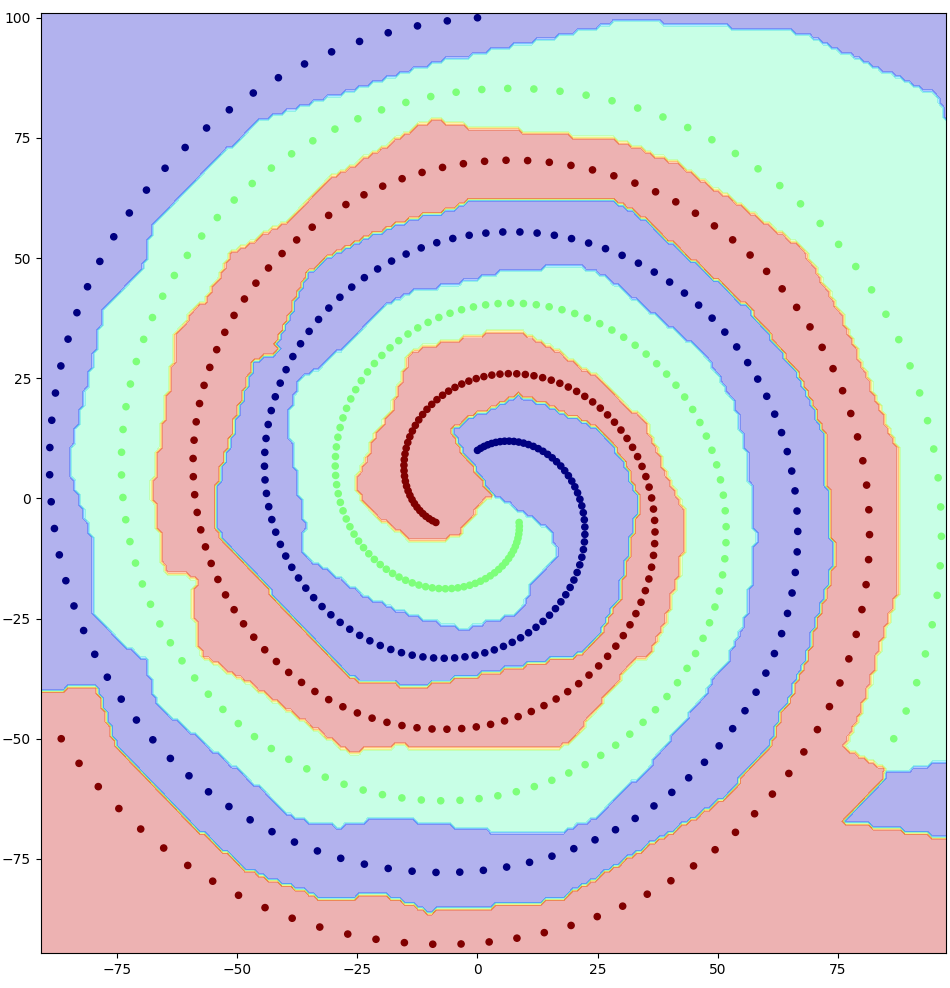
\includegraphics[width=5cm]{3spirals-decision_region.png} }}
    \qquad
    \subfloat[accuracy plot]{{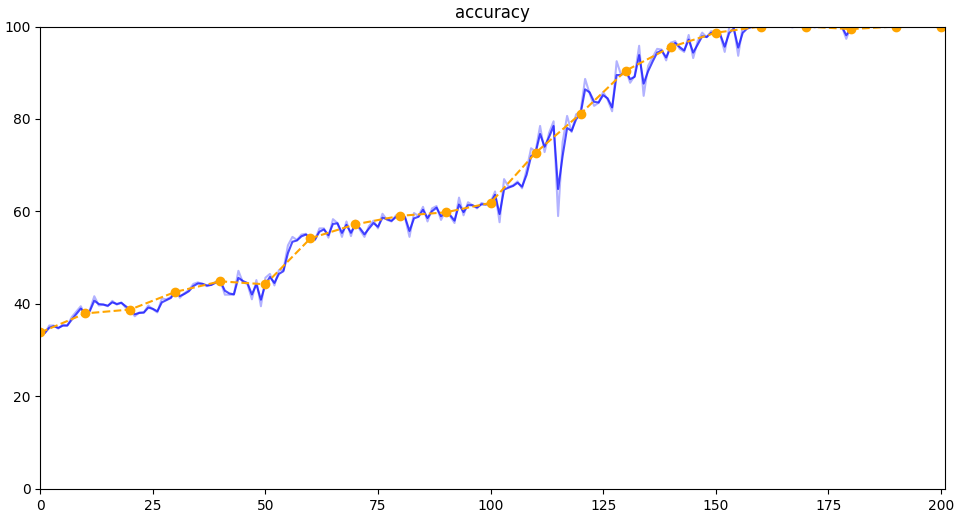
\includegraphics[width=7cm]{3spirals-acc.png} }}
    \qquad
    \subfloat[error plot]{{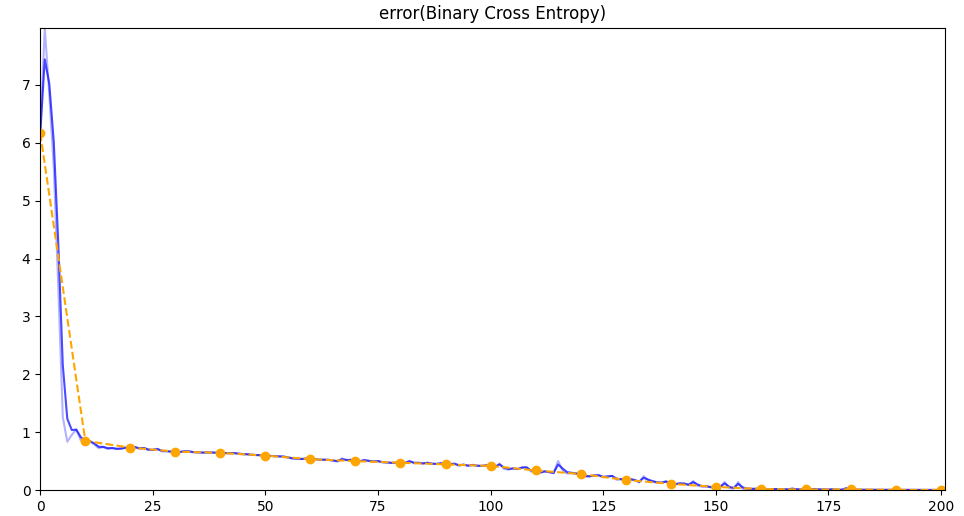
\includegraphics[width=7cm]{3spirals-err.png}}}
    \caption{3 spirals}
\end{figure}

\newpage
\subsection{7 Spirals with Advanced Model}
\subsubsection{Network Settings}
\begin{lstlisting}[language=Python]
# dataset
dataset = NSpirals(7)
dataset_num = 1000

# network
network_structure = [
    FullyConnected(2, 15, -1, 1),
    ReLu(0.1),
    FullyConnected(15, 15, -1, 1),
    ReLu(0.1),
    FullyConnected(15, 7, -1, 1),
    SoftMax()
]

# train
epochs = 2000
optimizer = Adam(0.006, 0.99)
loss = BinaryCrossEntropy()
\end{lstlisting}

\subsubsection{Network Settings}
\begin{figure}[!ht]
    \centering
    \subfloat[comparsion plot]{{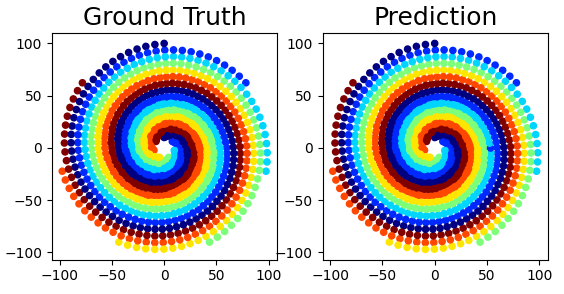
\includegraphics[width=10cm]{7spirals-gt_pd.png} }}
    \qquad
    \subfloat[decision region]{{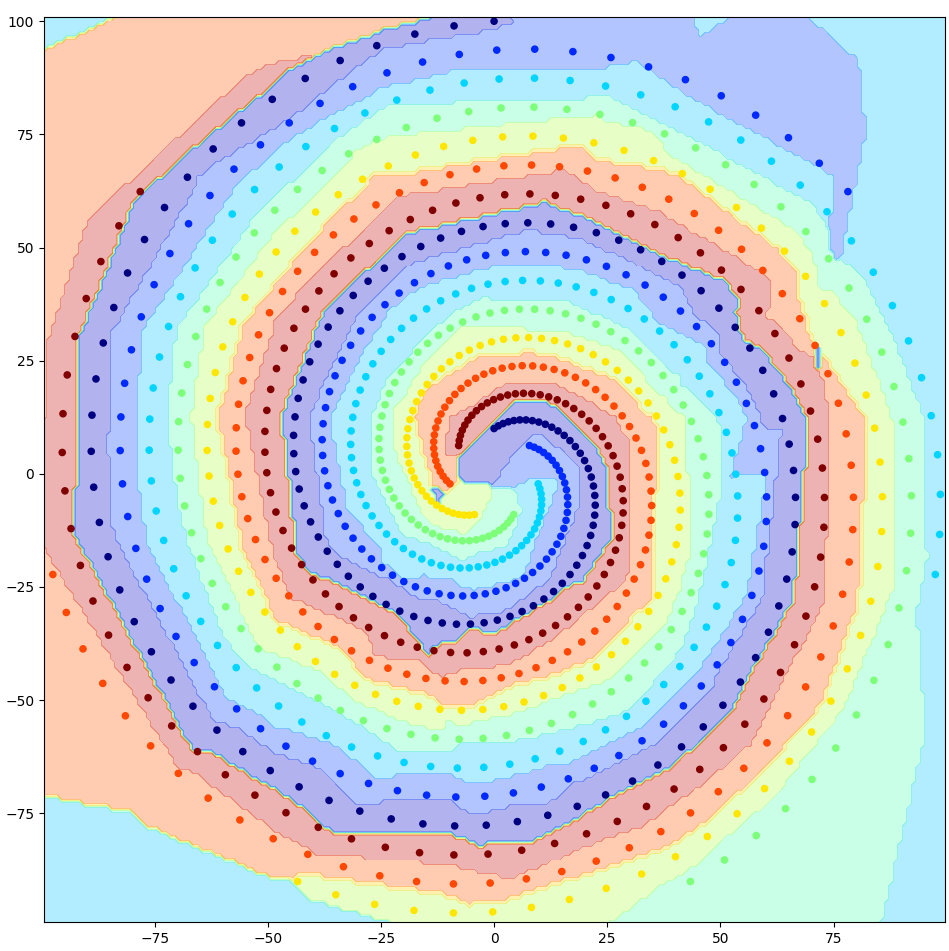
\includegraphics[width=5cm]{7spirals-decision_region.png} }}
    \qquad
    \subfloat[accuracy plot]{{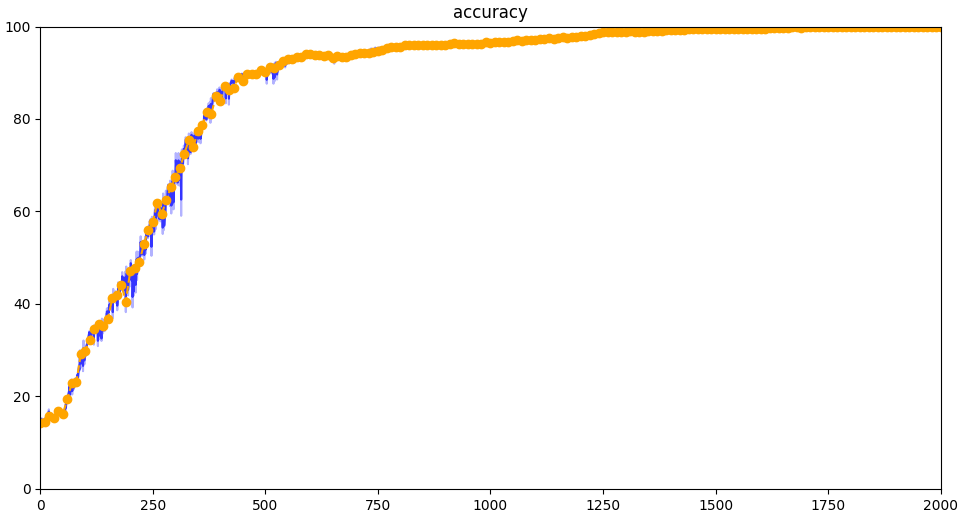
\includegraphics[width=7cm]{7spirals-acc.png} }}
    \qquad
    \subfloat[error plot]{{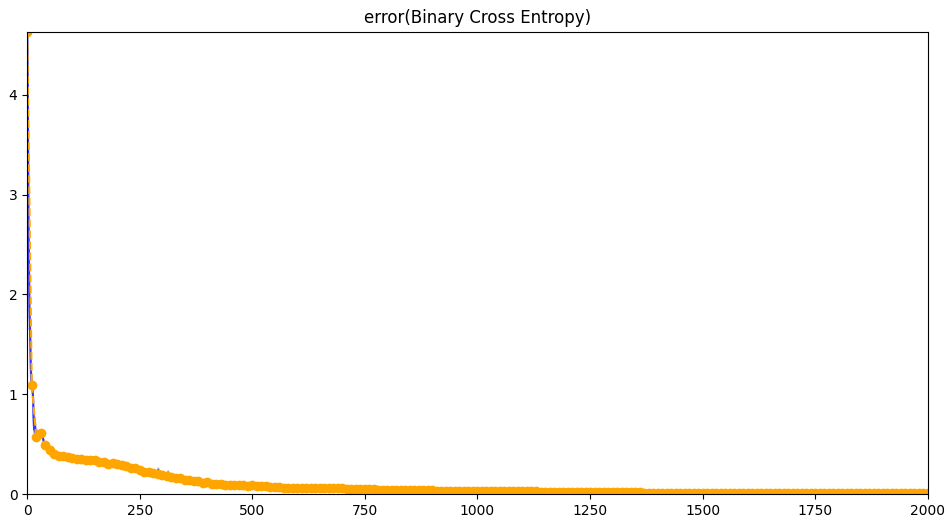
\includegraphics[width=7cm]{7spirals-err.png}}}
    \caption{7 spirals}
\end{figure}


\end{document}
